\documentclass[tikz,border=5pt]{standalone}
\usepackage{tikz}
\usetikzlibrary{calc}

\begin{document}
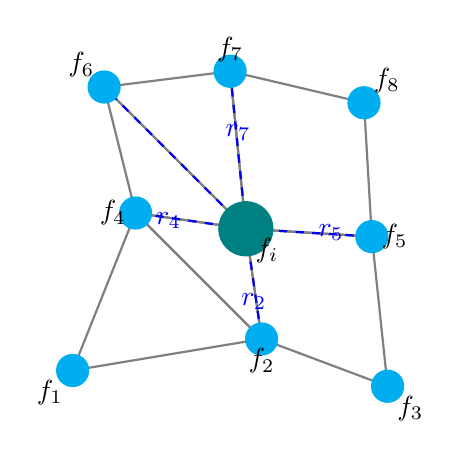
\begin{tikzpicture}[scale=2.0]

    % Define vertices of a triangular mesh region
    \coordinate (A) at (0,0);       % f_1
    \coordinate (B) at (1.2,0.2);   % f_2
    \coordinate (C) at (2.0,-0.1);  % f_3
    \coordinate (D) at (0.4,1.0);   % f_4
    \coordinate (E) at (1.1,0.9);   % f_i (central point)
    \coordinate (F) at (1.9,0.85);  % f_5
    \coordinate (G) at (0.2,1.8);   % f_6
    \coordinate (H) at (1.0,1.9);   % f_7
    \coordinate (I) at (1.85,1.7);  % f_8

    % Draw triangles (mesh edges)
    \draw[gray, thick] (A) -- (B) -- (D) -- cycle;
    \draw[gray, thick] (B) -- (C) -- (F) -- (E) -- cycle;
    \draw[gray, thick] (B) -- (E) -- (D) -- cycle;
    \draw[gray, thick] (D) -- (E) -- (G) -- cycle;
    \draw[gray, thick] (E) -- (H) -- (G) -- cycle;
    \draw[gray, thick] (E) -- (F) -- (I) -- (H) -- cycle;

    % Draw stencil connections (from central point to neighbors)
    \draw[blue, thick, dashed] (E) -- (B);
    \draw[blue, thick, dashed] (E) -- (D);
    \draw[blue, thick, dashed] (E) -- (F);
    \draw[blue, thick, dashed] (E) -- (H);
    \draw[blue, thick, dashed] (E) -- (G);

    % Distance labels
    \node[blue, below] at ($(E)!0.5!(B)$) {$r_2$};
    \node[blue, left] at ($(E)!0.5!(D)$) {$r_4$};
    \node[blue, right] at ($(E)!0.5!(F)$) {$r_5$};
    \node[blue, above] at ($(E)!0.5!(H)$) {$r_7$};

    % Neighbor points (cyan)
    \fill[cyan] (A) circle (3pt); \node[below left] at (A) {$f_1$};
    \fill[cyan] (B) circle (3pt); \node[below] at (B) {$f_2$};
    \fill[cyan] (C) circle (3pt); \node[below right] at (C) {$f_3$};
    \fill[cyan] (D) circle (3pt); \node[left] at (D) {$f_4$};
    \fill[cyan] (F) circle (3pt); \node[right] at (F) {$f_5$};
    \fill[cyan] (G) circle (3pt); \node[above left] at (G) {$f_6$};
    \fill[cyan] (H) circle (3pt); \node[above] at (H) {$f_7$};
    \fill[cyan] (I) circle (3pt); \node[above right] at (I) {$f_8$};

    % Central point (teal/dark cyan - larger)
    \fill[teal] (E) circle (5pt); \node[below right] at (E) {$f_i$};

\end{tikzpicture}
\end{document}
